\chapter{Methodology}

% mention how graffiti with light would not work, say why we opted for buildings

This chapter discusses the process of joining the several datasets and the pipeline we use to build the models. In total, eight datasets are used from the \href{https://opendata.vancouver.ca/pages/home/}{City of Vancouver Open Data Portal}. Some of these are updated weekly by the Vancouver authorities. Therefore, the versions we used were saved and uploaded on our \href{https://github.com/CowKeyMan/PredictingGraffitiUsingCityLayouts}{github}, to keep results consistent.

\section{Pre-processing}

The first two datasets we use are \textit{local-area-boundary}, which contains the geometry of the several regions of Vancouver, and \textit{buildings-footprints-2009}, which contains several information about buildings. The first step is to filter the buildings dataset. All the columns are removed except the building id, roof type, the highest elevation and the geometry. Several buildings share the same id, hence these are joined. When joining, the result has the maximum highest elevation, and the union of the two buildings as geometry. The count of the join is put into a new column called sub-buildings. Lastly, since some buildings outside of the Vancouver area were included in the dataset, a check is made such that if the geometry of the building does not fully intersect with a local area, then it is discarded.

Although this dataset contains useful information about the buildings, it does not contain some important information, namely the street and local area that the building lies in. To get these two fields, we join with \textit{property-addresses}. A property does not necessarily indicate a building, but merely a plot of land. Hence, to merge this dataset with our previous one, we join the coordinate of the properties with the geometry shape of the buildings. The properties are looped on each building and we merge with the first one whose coordinate intersects the geometry of the building.

The next step is to join with the \textit{graffiti} dataset in order to get the number of graffiti per building. This was done by joining on the coordinate of the graffiti and the coordinate of the property that the building was previously joined with. If we join with the coordinates rounded to five decimal places\footnote{five decimal places is precision needed to distinguish objects up to 1.1m apart from each other, for example, 2 trees}, every graffiti will lie on a property coordinate. However, since some properties were previously pruned due to joining, we unfortunately end up losing 27.6\% of the graffiti instances.

To extract more information from our data, we also include objects which are close to each building. In terms of distances, we estimate the approximate distance of one house, two houses and four houses, and include the features of nearby buildings into the features of the current one. The new features are called: \textit{one\_house\_away\_buildings\_count, one\_house\_away\_graffiti\_count, \ldots}. Then, we add features which are as far as the other distances, so we have \textit{two\_houses\_away\_buildings\_count, \ldots, four\_houses\_away\_street\_lights}. The full feature set can be seen in Appendix~\ref{app:all_model_features}. The street lights data comes from the \textit{street-lighting-poles} dataset. Since coordinates are used, geodesic distance would have been the most appropriate distance measure to use. However, since we are working with a very small area of the planet, the resulting intermediary data frames are close to identical when using euclidean distance. As a result, euclidean was used due to its lower computational cost, as projection turns out to be a very resource intensive process, especially if it needs to be done quadratically to the dataset.

Leaving the resultant previous dataset on hold, we do some processing on other smaller datasets which will be joined later. First, the \textit{local-area-boundary} and \textit{cencus2016} datasets are joined to obtain the area in meters squared, the population and the population density of each local area are extracted and put into a single dataset. The \textit{public-streets} dataset is also cleaned so that it will give us the type of each street, for example, whether the street is arterial or residential and a way to identify buildings on the same streets.

Finally, every dataset is joined together. Any Vancouver specific features are removed, such as local area and street names. The street and roof type features are one-hot encoded so we can build a model out of them. The full preprocessing pipeline can be visualised in Figure~\ref{fig:methodology}. Next, we discuss the pipeline used to build our regression and classification models.

\begin{figure}
   \centering
   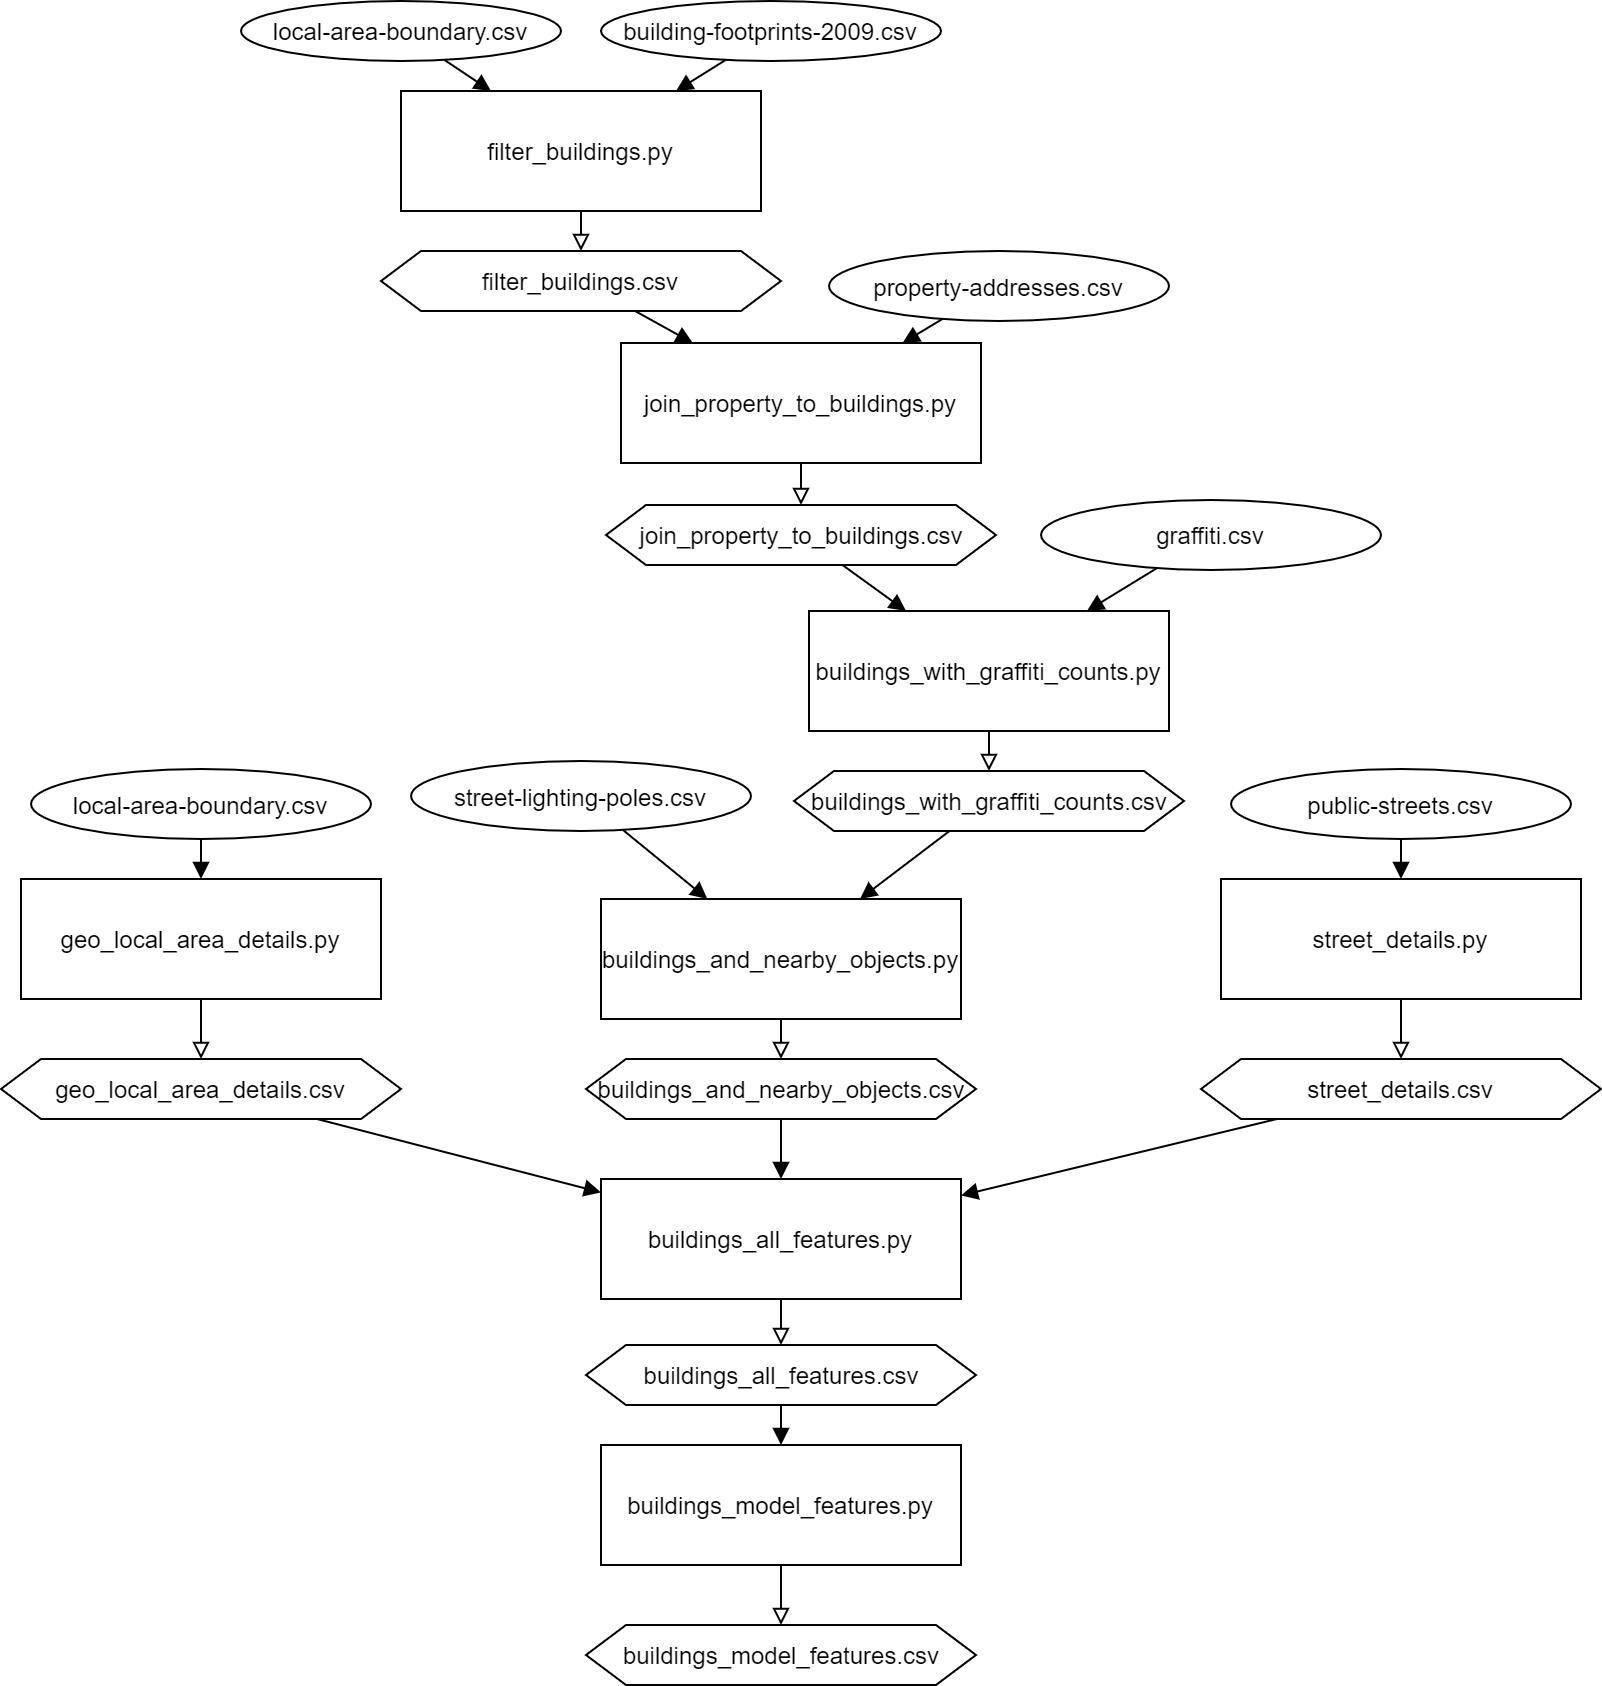
\includegraphics[width=\textwidth]{images/MethodologyInputOutputDiagram.png}
   \caption{Input output diagram. Notation: Oval = Original Data, Hexagon = Generated Data, Rectangle = Script, Filled Arrow = Input, Hollow Arrow = Output}
   \label{fig:methodology}
\end{figure}


\section{Models}

For our purposes, we train both regression and classification models. The target value for regression is the graffiti count for each building, while for classification we predict whether a building has or does not have graffiti on it. For each model that we build, the pipeline is the same. We first perform scaling and then perform hyper parameter tuning on a randomly selected 5000 samples of our dataset. For scaling, we scaled the continuous variables to mean 0 and standard deviation 1. Next, we split the full dataset into five folds and perform cross validation. A scaler is first fit on the train set, then we train the model. Afterwards, the scaler is applied to the test set, and finally the test set is passed through our model. For a listing of all the model parameters we tried, refer to Appendix~\ref{app:model_parameters}.

The results shown in the \href{https://cowkeyman.github.io/PredictingGraffitiUsingCityLayouts/results.html}{blog} are the averages of the results obtained by our models. Full results tables can be found in Appendix~\ref{app:full_results}. When it comes to explaining our models, we train separate linear models on our entire dataset. The entire dataset is then fed back into the model to receive the predictions based on the fitted parameters. Linear models were chosen for this task to minimize the risk of overfitting. These predictions were then used to generate heatmaps of the anticipated locations where new graffiti might appear.

